\documentclass[9pt,a4paper]{extarticle}\usepackage[]{graphicx}\usepackage[]{color}
%% maxwidth is the original width if it is less than linewidth
%% otherwise use linewidth (to make sure the graphics do not exceed the margin)
\makeatletter
\def\maxwidth{ %
  \ifdim\Gin@nat@width>\linewidth
    \linewidth
  \else
    \Gin@nat@width
  \fi
}
\makeatother

\definecolor{fgcolor}{rgb}{0.345, 0.345, 0.345}
\newcommand{\hlnum}[1]{\textcolor[rgb]{0.686,0.059,0.569}{#1}}%
\newcommand{\hlstr}[1]{\textcolor[rgb]{0.192,0.494,0.8}{#1}}%
\newcommand{\hlcom}[1]{\textcolor[rgb]{0.678,0.584,0.686}{\textit{#1}}}%
\newcommand{\hlopt}[1]{\textcolor[rgb]{0,0,0}{#1}}%
\newcommand{\hlstd}[1]{\textcolor[rgb]{0.345,0.345,0.345}{#1}}%
\newcommand{\hlkwa}[1]{\textcolor[rgb]{0.161,0.373,0.58}{\textbf{#1}}}%
\newcommand{\hlkwb}[1]{\textcolor[rgb]{0.69,0.353,0.396}{#1}}%
\newcommand{\hlkwc}[1]{\textcolor[rgb]{0.333,0.667,0.333}{#1}}%
\newcommand{\hlkwd}[1]{\textcolor[rgb]{0.737,0.353,0.396}{\textbf{#1}}}%
\let\hlipl\hlkwb

\usepackage{framed}
\makeatletter
\newenvironment{kframe}{%
 \def\at@end@of@kframe{}%
 \ifinner\ifhmode%
  \def\at@end@of@kframe{\end{minipage}}%
  \begin{minipage}{\columnwidth}%
 \fi\fi%
 \def\FrameCommand##1{\hskip\@totalleftmargin \hskip-\fboxsep
 \colorbox{shadecolor}{##1}\hskip-\fboxsep
     % There is no \\@totalrightmargin, so:
     \hskip-\linewidth \hskip-\@totalleftmargin \hskip\columnwidth}%
 \MakeFramed {\advance\hsize-\width
   \@totalleftmargin\z@ \linewidth\hsize
   \@setminipage}}%
 {\par\unskip\endMakeFramed%
 \at@end@of@kframe}
\makeatother

\definecolor{shadecolor}{rgb}{.97, .97, .97}
\definecolor{messagecolor}{rgb}{0, 0, 0}
\definecolor{warningcolor}{rgb}{1, 0, 1}
\definecolor{errorcolor}{rgb}{1, 0, 0}
\newenvironment{knitrout}{}{} % an empty environment to be redefined in TeX

\usepackage{alltt}
\usepackage{f1000_styles}
\usepackage{hyperref}
\usepackage{todonotes}

\usepackage{tabularx}

%% Default: numerical citations
\usepackage[numbers]{natbib}

%% Uncomment this lines for superscript citations instead
% \usepackage[super]{natbib}

%% Uncomment these lines for author-year citations instead
% \usepackage[round]{natbib}
% \let\cite\citep
\IfFileExists{upquote.sty}{\usepackage{upquote}}{}
\begin{document}

\pagestyle{front}

\title{\textit{BiocPkgTools}: Toolkit for Mining the \emph{Bioconductor} Package Ecosystem}

\author[1]{Shian Su}
\author[2]{Vincent~J. Carey}
\author[3]{Lori Shepherd}
\author[1]{Matthew Ritchie}
\author[3]{Martin~T. Morgan}
\author[4]{Sean Davis}
\affil[1]{Molecular Medicine Division, The Walter and Eliza Hall Institute of Medical Research, Parkville, Australia}
\affil[2]{Channing Division of Network Medicine, Brigham and Women's Hospital, Boston, MA, USA}
\affil[3]{Roswell Park Comprehensive Cancer Center, Buffalo, NY, USA}
\affil[4]{Center for Cancer Research, National Cancer Institute, National Institutes of Health, Bethesda, MD, USA}

\maketitle
\thispagestyle{front}


\begin{abstract}
  \\ \textbf{Motivation:} The \emph{Bioconductor} project, a large
  collection of open source software for the comprehension of
  large-scale biological data, continues to grow with new packages
  added each week, motivating the development of software tools
  focused on exposing package metadata to developers and users. The
  resulting BiocPkgTools package facilitates access to extensive
  metadata in computable form covering the \emph{Bioconductor} package
  ecosystem, facilitating downstream applications such as custom
  reporting, data and text mining of \emph{Bioconductor} package text
  descriptions, graph analytics over package
  dependencies, and custom search approaches. \\
  \textbf{Results:} The BiocPkgTools package has been incorporated
  into the \emph{Bioconductor} project, installs using standard
  procedures, and runs on any system supporting R. It provides
  functions to load detailed package metadata, longitudinal package
  download statistics, package dependencies, and \emph{Bioconductor}
  build reports, all in ``tidy data'' form. BiocPkgTools can convert
  from tidy data structures to graph structures, enabling graph-based
  analytics and visualization. An end-user-friendly graphical package
  explorer aids in task-centric package discovery. Full documentation
  and example use cases are included. \\ \textbf{Availability:} The
  BiocPkgTools software and complete documentation are available from
  \emph{Bioconductor}
  (\href{https://bioconductor.org/packages/BiocPkgTools}{https://bioconductor.org/packages/BiocPkgTools}).
\end{abstract}

\section*{Keywords}

Bioconductor, data mining, R, open data, software, data science, software development, bioinformatics






\clearpage
\pagestyle{main}

\section*{Introduction}

\emph{Bioconductor} is a open source software project (comprising
1741 individual analysis packages) and community for
the analysis and comprehension of large-scale biological data. Newly
submitted software packages undergo a technical review to ensure that
best practices and \emph{Biocondutor} coding conventions are
followed. The project maintains an automated build system that ensures
that packages in the \emph{Bioconductor} project are compiled and
built successfully and pass basic checks. Package downloads are
tracked and aggregated by package and month, longitudinally. Finally,
package details such as title, description, version, author, and
dependencies on other R packages are compiled based on package
metadata.

The current size and growth of the \emph{Bioconductor} project suggests that
there is merit in exposing computable forms of the metadata describing
the \emph{Bioconductor} package ecosystem. To that end, we developed a small
suite of tools to provide easy access to project details such as download
statistics, bulk package metadata, and package build
status. Developers, project leaders, open source software researchers,
and \emph{Bioconductor} end users can build on the availability of these data
for applications such as custom reporting, dependency graph analytics,
package filtering, and text mining.


\section*{Features and usage}

The core functionality of BiocPkgTools is to expose
\emph{Bioconductor} project and package metadata as tidy data
\citep{Wickham2014-ye} objects. The data presented by the package are
accessed directly from online resources available from
\emph{Bioconductor}. As such, the package relies on web connectivity and
collects the most recent data. Installation instructions are detailed
on the package website.

Package functionality can be roughly divided into data access, data
presentation, and graph/network functionality. See Table
\ref{tab:functions} for an overview.

\begin{figure}
  \caption{Schematic overview of the BiocPkgtools package. BiocPkgTools can access and transform web-accessible resources including package metadata, download statistics, dependencies between packages, and updated \emph{Bioconductor} build report status to "tidy data" reports that can be manipulated using standard R tools. Interactive package exploration is also available.}
  \label{fig:overview}
  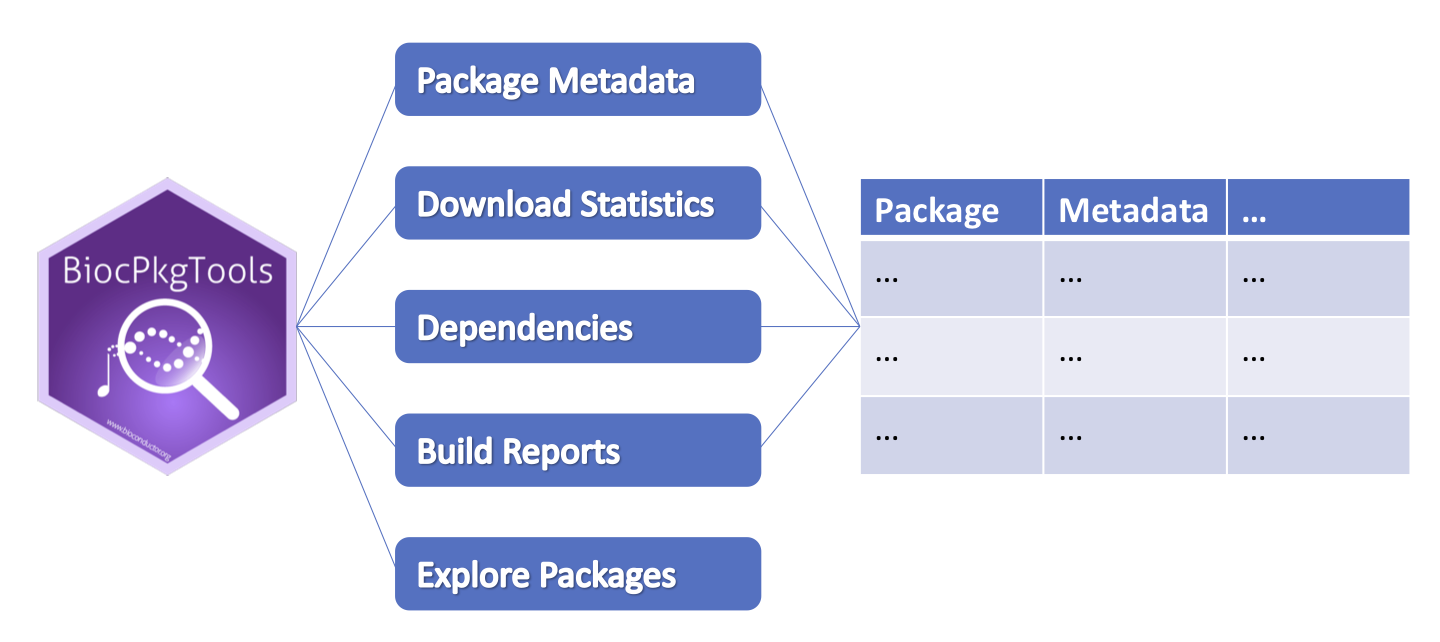
\includegraphics[width=1.0\textwidth]{BiocPkgToolsFig1mock.png}
\end{figure}


\begin{table}[h]
  \caption{Main package functions and descriptions.}
  \label{tab:functions}
  \begin{tabularx}{\linewidth}{ l X }
    \hline
    Name & Functionality \\
    \hline
    biocPkgList & Package details including description, author and maintainer, dependencies, URLs, bug report mechanism \\
    biocDownloadStats & Monthly download statistics for all packages \\
    biocbuildReport & \emph{Bioconductor} build report for all packages and systems \\
    biocExplore & Interactive, browsable ``bubble plot'' of \emph{Bioconductor} packages and details \\
    problemPage & Interactive, customized build report for an individual package author \\
    buildPkgDependencyDataFrame & Package dependencies as data frame \\
    buildPkgDependencyIgraph & Package dependencies as a graph \citep{igraph} \\
    inducedSubgraphByPkgs & Create a minimal subgraph of \emph{Bioconductor} dependencies based on specific packages \\
    subgraphByDegree & Create a subgraph of all packages within a given degree of a single package \\
    \hline
  \end{tabularx}
\end{table}

After installing BiocPkgTools, the \texttt{biocDownloadStats} function
can generate a tidy data structure summarizing monthly download
statistics (both total and unique IP addresses) for all \emph{Bioconductor}
packages.

\begin{knitrout}\small
\definecolor{shadecolor}{rgb}{0.969, 0.969, 0.969}\color{fgcolor}\begin{kframe}
\begin{alltt}
\hlkwd{library}\hlstd{(BiocPkgTools)}
\hlstd{dlstats} \hlkwb{=} \hlkwd{biocDownloadStats}\hlstd{()}
\hlkwd{head}\hlstd{(dlstats,} \hlnum{3}\hlstd{)}
\end{alltt}
\begin{verbatim}
## # A tibble: 3 x 6
##   Package  Year Month Nb_of_distinct_IPs Nb_of_downloads repo    
##   <fct>   <int> <fct>              <int>           <int> <chr>   
## 1 ABarray  2018 Jan                  117             150 Software
## 2 ABarray  2018 Feb                   97             125 Software
## 3 ABarray  2018 Mar                  102             121 Software
\end{verbatim}
\end{kframe}
\end{knitrout}

The \texttt{biocBuildReport} function gathers information from the
\emph{Bioconductor}
\href{http://bioconductor.org/checkResults/release/bioc-LATEST/}{build
  report site} and can be used, for example, to summarize the ``build
status'' for all \emph{Bioconductor} pacakages.

\begin{knitrout}\small
\definecolor{shadecolor}{rgb}{0.969, 0.969, 0.969}\color{fgcolor}\begin{kframe}
\begin{alltt}
\hlstd{buildrep} \hlkwb{=} \hlkwd{biocBuildReport}\hlstd{(}\hlkwc{version} \hlstd{=} \hlstr{"3.9"}\hlstd{)}
\hlkwd{table}\hlstd{(buildrep}\hlopt{$}\hlstd{stage, buildrep}\hlopt{$}\hlstd{result)}
\end{alltt}
\begin{verbatim}
##           
##            ERROR   OK skipped TIMEOUT WARNINGS
##   buildbin     2 3352      70       0        0
##   buildsrc    93 5057       0       5        0
##   checksrc    57 4181      98       8      811
##   install     39 5116       0       0        0
\end{verbatim}
\end{kframe}
\end{knitrout}

These data are useful to developers to track the health of their
software either programmatically or via a searchable, sortable table
from the \texttt{problemPage} function.

As an alternative to basic web browser search and the
\emph{Bioconductor} online software list, the \texttt{biocExplore}
function offers interactive and graphical approach to package browsing
(see Figure \ref{fig:biocexplore}). The biocExplore widget allows browsing
packages under different biocViews, Bioconductor's software catergory tags. This
interactively visualises the relative number of downloads each package has under
different biocViews, allowing users to quickly determine which packages are most
commonly used for different analysis tasks.

\begin{figure}
  \includegraphics[width=\linewidth]{biocExplore}
  \caption{The \texttt{biocExplore} function opens an interactive web application that allows users to select focused groups of \emph{Bioconductor} packages to view as a bubble plot. Bubbles are sized based on download statistics. Hovering over a bubble will give download number while clicking on a bubble will pop up a package details page, including a link to the package landing page.}
  \label{fig:biocexplore}
\end{figure}

The \emph{Bioconductor} package ecosystem is, by design, highly
interconnected via package dependencies. Several functions in the
BiocPkgTools package provide examples of package dependency graph
creation and visualization. Figure \ref{fig:dependencygraph} displays
packages within one degree of dependency relationship of the GEOquery
package.

\begin{figure}
  \includegraphics[width=\linewidth]{BiocPkgToolsDependencyGraph}
  \caption{The \texttt{subgraphByDegree} function builds a data
    visualization of dependencies between all packages within one
    degree of the GEOquery package using the visNetwork package
    \citep{visNetwork}. Links are colored based on type (Suggests [light blue],
    Depends [green], and Imports [red]) and arrows point to the ``dependent''
    package. }
  \label{fig:dependencygraph}
\end{figure}

\section*{Implementation}

BiocPkgTools is implemented as a standard R package and hosted in the
\emph{Bioconductor} repository. All functions are documented and include
examples. An included tutorial (vignette) demonstrates features and
capabilities.

\section*{Data availability} % Optional - only if novel data or analyses are included
All data accessed and used by the BiocPkgTools package are publicly available and are updated regularly at the \emph{Bioconductor} project.

\section*{Software availability}
This section will be generated by the Editorial Office before publication. Authors are asked to provide some initial information to assist the Editorial Office, as detailed below.
\begin{itemize}
\item Software URL: \href{https://bioconductor.org/packages/BiocPkgTools}{https://bioconductorg.org/packages/BiocPkgTools}
\item Version Control URL: \href{https://github.com/seandavi/BiocPkgTools}{https://github.com/seandavi/BiocPkgTools}
\item Software package DOI: \href{https://doi.org/doi:10.18129/B9.bioc.BiocPkgTools}{doi:10.18129/B9.bioc.BiocPkgTools}
\item Software License: MIT License
\end{itemize}



\section*{Author contributions}
SD conceived of the project. All authors have reviewed and edited the manuscript. Authors contributing to code include MM, SD, SS, LS, and VC.


\section*{Competing interests}
No competing interests were disclosed.

\section*{Grant information}

Research reported in this publication was supported by the National
Human Genome Research Institute of the National Institutes of Health
under award number U41HG004059, the National Cancer Institute of the
National Institutes of Health under award numbers U24CA180996 and
U01CA214846-02, and the Center for Cancer Research, part of the
Intramural Research Program at the National Cancer Institute at the
National Institutes of Health. Part of this work was performed on
behalf of the SOUND Consortium and funded under the EU H2020
Personalizing Health and Care Program, Action contract number 633974.


\bibliographystyle{natbib}
%\bibliographystyle{achemnat}
%\bibliographystyle{plainnat}
%\bibliographystyle{abbrv}
%\bibliographystyle{bioinformatics}
%
%\bibliographystyle{plain}
%
\bibliography{references}

\end{document}
